% !TEX root = ../../../main.tex
% 来源：中学数学实验教材·第三册（高中数学）
% 章节：二次函数 / 二次函数
% 原始文件：5.tex，行 351-373
% 类型：tikz
% ---
    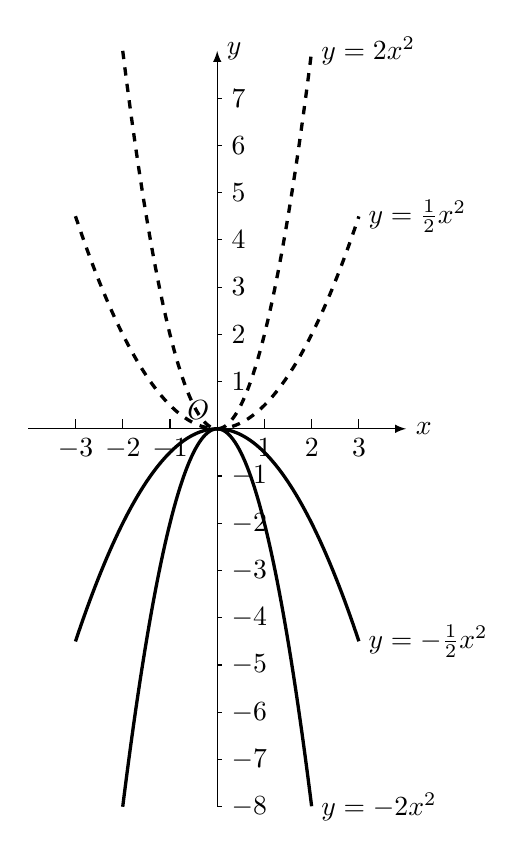
\begin{tikzpicture}[>=latex, scale=.6]
\draw[->] (-4,0)--(4,0)node[right]{$x$};
    \draw [->] (0,-8)--(0,8)node[right]{$y$};
\foreach \y in {-8,-7,...,-1,1,2,...,7}
{
    \draw (0,\y)--(.1,\y)node[right]{$\y$};
}
\foreach \x in {-3,-2,-1,1,2,3}
{
    \draw (\x,0)node[below]{$\x$}--(\x,.2);
}

\draw [domain=-3:3, samples=100, very thick, dashed]plot(\x,{\x*\x*0.5});
\draw [domain=-2:2, samples=100, very thick, dashed]plot(\x,{\x*\x*2});

\draw [domain=-3:3, samples=100, very thick]plot(\x,{-\x*\x*0.5});
\draw [domain=-2:2, samples=100, very thick]plot(\x,{-\x*\x*2});
\node at (-.4,.4){$O$};
\node at (2,8)[right]{$y=2x^2$};
\node at (3,4.5)[right]{$y=\frac{1}{2}x^2$};
\node at (2,-8)[right]{$y=-2x^2$};
\node at (3,-4.5)[right]{$y=-\frac{1}{2}x^2$};      
    \end{tikzpicture}
